\section{Tworzenie silnika szachowego}\label{sec:tworzenie silnika szachowego}

\begin{frame}{Reprezentacja szachownicy i generowanie ruchów}

    \begin{columns}
        \column{0.45\textwidth}
        \begin{block}{Reprezentacja szachownicy}
            \begin{itemize}
                \item Tablica pól szachowych
                \item Tablice bitowe bierek
            \end{itemize}
            \centering {
                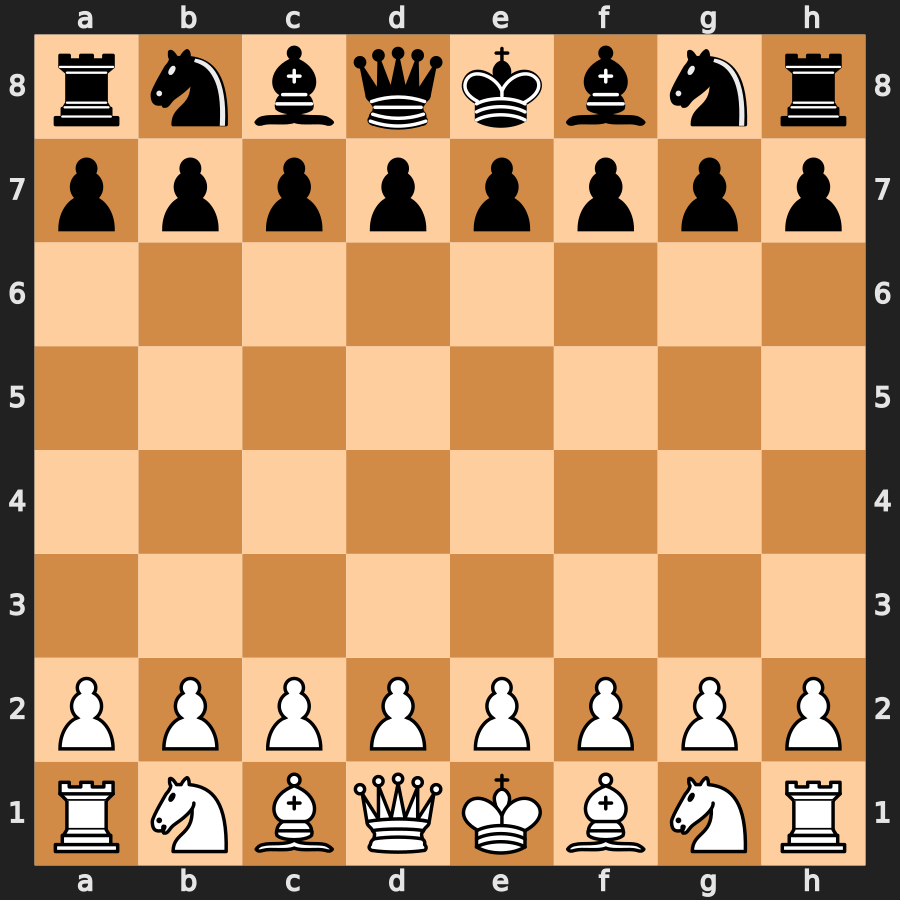
\includegraphics[width=0.8\textwidth]{rysunki/pozycja_startowa}
            }
        \end{block}
        \column{0.55\textwidth}

        \begin{block}{Generowanie ruchów pionów}
                    $moves & = empty$ \\
                    $moves & = moves \wedge (pionki_w\ll16)$ \\
                    $moves & = moves \wedge (empty\ll8)$ \\
                    $moves & = moves \wedge rank4$ \\
        \end{block}

        \begin{block}{Hyperbola Quintessence}
            $linia = (o-2r) \oplus \Bigr[( o'-2r')\Bigl]'$
        \end{block}

    \end{columns}
\end{frame}

\begin{frame}{Wyszukiwanie i ewaluacja}
    \begin{columns}
        \column{0.5\textwidth}
        \begin{block}{Algorytym wyszukiwania}
            \begin{enumerate}
                \item Gra dwuosobowa
                \item Gra o sumie stałej
                \item Postać ekstensywna
                \item Gra skończona
                \item Gra o doskonałej informacji
            \end{enumerate}

        \end{block}

        \begin{alertblock} {Gra ściśle konkurencyjna}
            Aby uzyskać maksymalną wypłatę, gracz dąży do tego, by~zminimalizować sumę wypłat
            przeciwnika.
        \end{alertblock}

        \column{0.5\textwidth}

        \centering {
            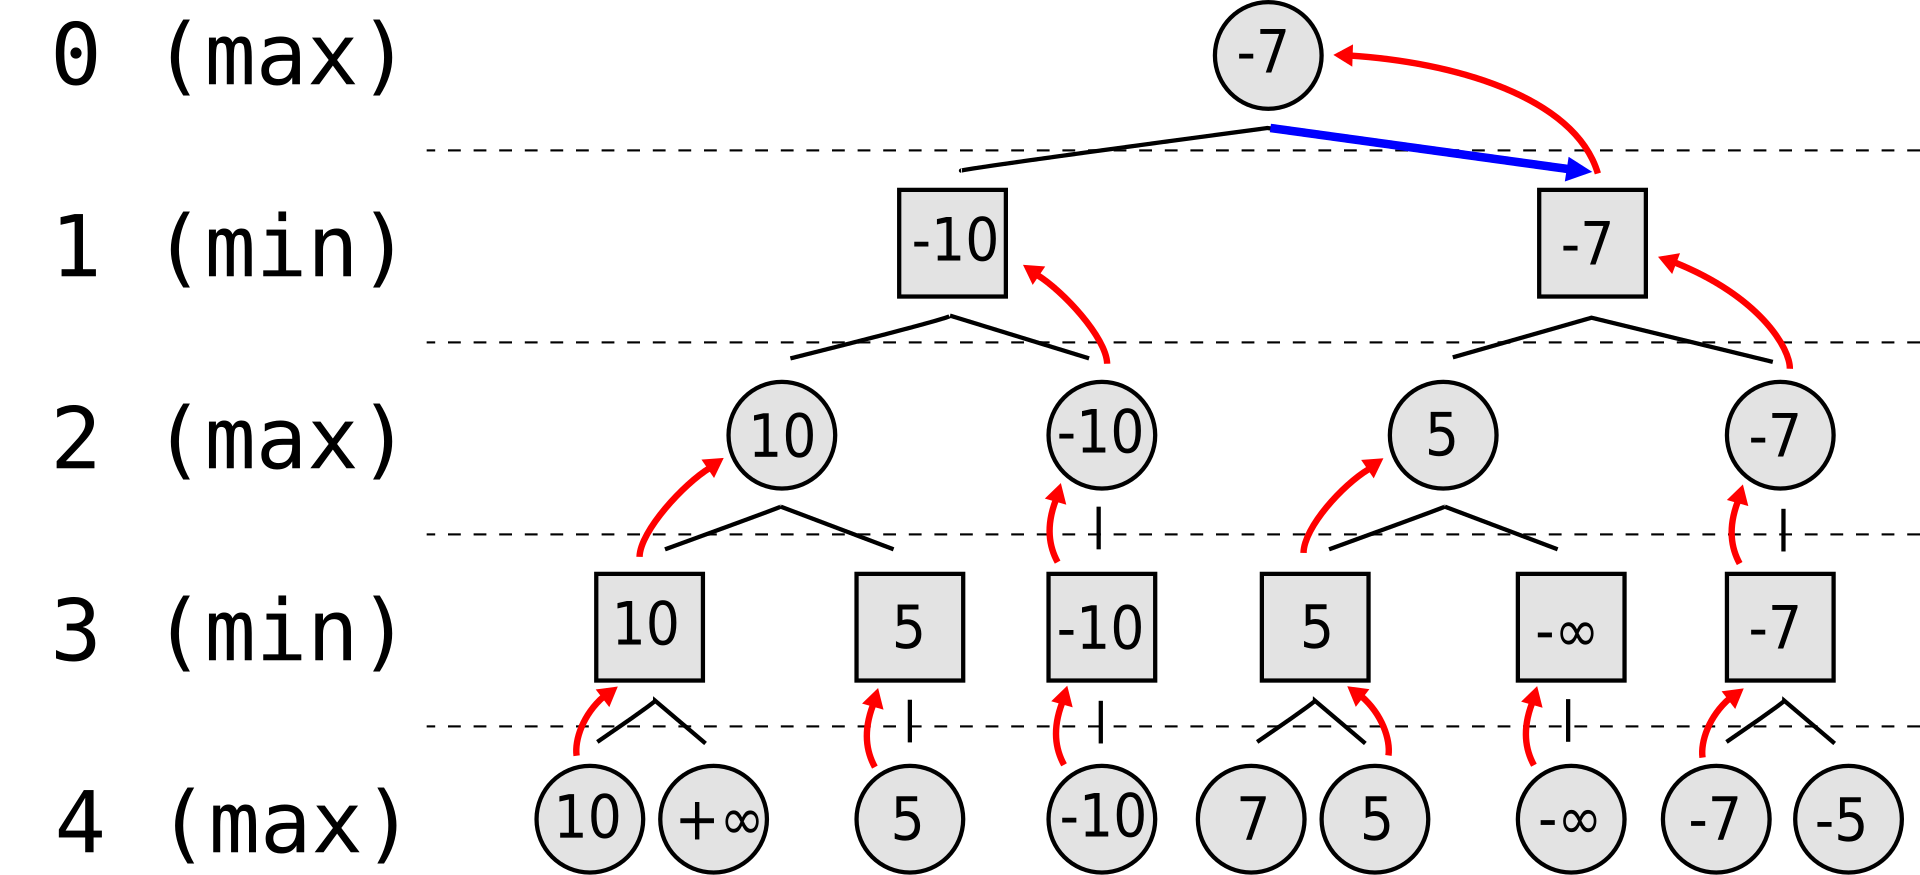
\includegraphics[width=1\textwidth]{rysunki/minimax}
        }

        \begin{block}{Ocena heurystyczna}
            \begin{itemize}
                \item Ocena stanu gry
                \item Wartość bierek
            \end{itemize}
        \end{block}

    \end{columns}
\end{frame}